\documentclass[letterpaper,10pt,onecolumn]{article}

\usepackage{setspace} 
\singlespacing
\usepackage{graphicx}                                        
\usepackage{amssymb}                                         
\usepackage{amsmath}                                         
\usepackage{amsthm}
\usepackage{mathtools}
\usepackage{algorithmic}
\usepackage{url}
\usepackage{tikz}         
\usetikzlibrary{matrix}
\usepackage{listings}
\usepackage{tabu}
\usepackage{mathptmx}
\usepackage{fullpage}
\usepackage{enumerate}
\usepackage{fancyvrb}
                             

%%%
%%% Formatting details
%%%
\sloppy
\sloppypar
\widowpenalty=0
\clubpenalty=0
\displaywidowpenalty=0
\raggedbottom
\pagestyle{plain}

\DefineVerbatimEnvironment{program}{Verbatim}
  {baselinestretch=1.0,xleftmargin=5mm,fontsize=\small,samepage=true}

\def\denseitems{
    \itemsep1pt plus1pt minus1pt
    \parsep0pt plus0pt
    \parskip0pt\topsep0pt}

\newcommand{\prog}[1]{{\small\texttt{#1}}}

\newcommand{\tagtree}[3]{#1 \langle #2, #3 \rangle}

\usepackage{geometry}
\geometry{textheight=9.5in, textwidth=7in}
\parindent = 0.0 in
\parskip = 0.1 in
\title{Imperative Programming with Variational Effects}
\author{Alex Grasley}
\begin{document}

\maketitle

\section{Introduction}

%% TODO

\section{Background}

\subsection{The choice calculus}

In order to formally represent choices in our programs we employ the choice
calculus \cite{ericthesis,erwig2011choice}. The fundamental unit of the choice calculus is
the \emph{choice}, which is a set of values called \emph{alternatives}.
There are many data structures that can be used to model
choices, but for our purposes we utilize a data structure we refer
to as a formula tree \cite{walkingshaw2014projectional,walkingshaw2014variational}.
Formula trees represent the set of alternatives as a binary tree, with concrete
values at the leaves of the tree. Each node of the tree is tagged with a formula from a boolean
algebra consisting of boolean literals, variables, negation, conjunction, and disjunction. We call these
tags the \emph{dimensions} of the choices. Notationally we represent these choice trees
via angle brackets. For example, a choice in dimension $A$ (where $A$ is a boolean variable)
between the values $1$ and $2$ is written $\tagtree{A}{1}{2}$.

Each boolean variable in a dimension can be viewed as coding for the presence or absence of a
particular feature that we wish to vary. To continue the above example, $\tagtree{A}{1}{2}$
represents a variational value that is $1$ when feature $A$ is present and $2$ otherwise. Because
dimensions can be any expression from a boolean algebra, we can combine them in a way
analogous to conditional expressions. For example, the choice $\tagtree{(A \wedge \neg B)}{1}{2}$
is a value that represents $1$ when feature $A$ is present and $B$ is absent, and $2$ otherwise.

The \emph{selection} operation on a choice can be used to eliminate dimensions. We define a function
\emph{sel} that takes a \emph{selector} and a variational value and eliminates dimensions based off
of the selector. For formula trees selectors are also booleans formulas, and can be seen as specifying
a condition that is assumed to hold true. Therefore, for a given dimension and
selector, we eliminate the choice and replace it with the left branch if the selector logically implies
the truth of the dimension. Similarly, if the selector logically implies the falsehood of the dimension, we eliminate the choice
and replace it with the right branch. If neither implication is valid, the choice remains untouched with
both alternatives left intact.

It is often helpful to see this selection operation in action. The operation
$\mathit{sel}(A,\tagtree{A}{1}{2})$, can be seen as encoding the presence of feature $A$, which
will therefore produce the value $1$ as a result. Similarly, $\mathit{sel}(\neg A,\tagtree{A}{1}{2})$ can be seen as encoding the absence of feature $A$ and will
produce the value $2$. $\mathit{sel}(B,\tagtree{A}{1}{2})$ will result in an unchanged variational
value $\tagtree{A}{1}{2}$ because the selector $B$ does not logically imply either the truth or falsehood
of dimension $A$.

Selection is \emph{synchronized} for a given
dimension, meaning that two choices in the same value or expression that share a dimension must always
select the same alternative. For example, in the expression $\tagtree{A}{1}{2}+\tagtree{A}{3}{4}$,
the only possible selections are $1+3$ and $2+4$, while $1+4$ and $2+3$ can never occur due
to synchronization.

We say that a choice is $configured$ when all dimensions
have been eliminated, yielding a plain value without choices. We call these resulting plain values
\emph{variants}. We define a function \emph{conf} which takes a
\emph{configuration} and a variational value and produces a variant. Under the view of boolean
variables in dimensions as representing distinct features, a configuration for a formula tree gives
an assignment for each variable present in the dimensions of the variational value being configured.
A simple way to do this is to define a configuration as a list of the features that are present, with all
other features assumed to be absent. In other words, configurations are a list of variables that should
evaluate to true, will all other variables evaluating to false. Configuring a formula tree is then simply evaluating
each dimension given the variable assignment. If the dimension evaluates to true, then the left variant
is chosen, otherwise the right variant is chosen.

Using boolean formulas as our dimensions provides several advantages. For example, we can simplify trees like
$\tagtree{B}{1}{\tagtree{A}{1}{2}}$ to the more compact form $\tagtree{(B \vee A)}{1}{2}$. This is just
one of a number of optimizations that are made possible by representing dimensions as formulas
\cite{walkingshaw2014projectional,hubbard2016formula}. Formula choices are also more convenient
for maintaining a variational context during execution of a program, a fact that will become
more relevant when we present our work on variational imperative programming later in
this work. Despite these advantages, formulas incur some cost by introducing boolean
satisfiability problems into many common operations, which is an NP-complete problem. However, thanks to improvements in the
efficiency of modern SAT solvers, often the worst-case NP-complete performance of these satisfiability
problems can be avoided.

\subsection{Implementation of Formula Trees}

When integrating formula trees into an existing non-variational language we can choose to
either embed choices directly into the abstract syntax of the host language or utilize a type-generic
implementation. In this work we employ both strategies, opting to embed choices directly when dealing
with programs, while using the type-generic implementation for the values produced by those programs.
Here we present the type-generic implementation, although the basic principles explored here apply
equally to embedded representations.

Generic formula trees can be represented by the following Haskell datatypes:

\begin{program}
type Var = String
data Dim =
    Lit Bool
  | Ref Var
  | Not Dim
  | And Dim Dim
  | Or Dim Dim

data FTree a = One a | Chc Dim (FTree a) (FTree a) 
\end{program}

The datatype \prog{Dim} represents expressions in our boolean algebra, with variable names as strings.
The constructor \prog{One} creates the leaves of a formula tree, while \prog{Chc} creates the nodes.

This type-generic representation allows us to easily define some useful algebraic properties of
formula trees via typeclasses. Specifically, formula trees readily support implementation of the
Functor, Applicative, and Monad typeclasses:

\begin{program}
instance Functor FTree where
  fmap f (One a) = One (f a)
  fmap f (Chc d l r) = Chc d (fmap f l) (fmap f r)
  
instance Applicative FTree where
  pure = One
  (One f) <*> v = fmap f v
  (Chc d l r) <*> v = Chc d (l <*> v) (r <*> v)
  
instance Monad FTree where
  return = One
  (One v) >>= f = f v
  (Chc d l r) >>= f = Chc d (l >>= f) (r >>= f)
\end{program}

Astute readers will note that because formula trees are merely a special class of binary tree with
labeled nodes they share identical instances. The usefulness of defining these instances will be made
apparent further on in this work during the discussion of pure, side-effect free variational languages.

\subsection{Properties of choices}

% sharing is desirable. what is sharing?
The choice calculus gives us several desirable properties for variational programs.
The first is \emph{sharing}. A naive approach to executing a variational program is simply to
configure the variational program in order to produce each variant and run them all sequentially.
For a program with $n$ features this results in $2^n$ variants that must be executed. Crucially,
the naive approach must recompute any common elements shared between variants. Embedding
choices in our program, combined with a variability-aware model of execution allows us to exploit this
inherent sharing by only computing shared components once, greatly improving the efficiency of
executing a variational program.

% correctness and the commuting diagram
Another property of choices and variation that we are interested in is \emph{correctness}. In order
to take advantage of the benefits of sharing, we must develop a variability-aware model of execution
that produces variational values as its result. In order to determine whether our variational results
are correct we need a way to relate them back to the individual variants they represent.

Given a function $f : T \rightarrow U$ and its variational counterpart $g : V \rightarrow W$, we say that
the relationship between the two is correct if for some configuration $c$ the following equality holds:
$\mathit{conf}\ c \circ g = f \circ \mathit{conf}\ c$ \cite{hubbard2016formula}. Put simply, configuring the result
of passing a variational value to a variational function should be the same as pre-configuring the input
and the function itself. This can be visualized as the following commuting diagram:

\begin{center}
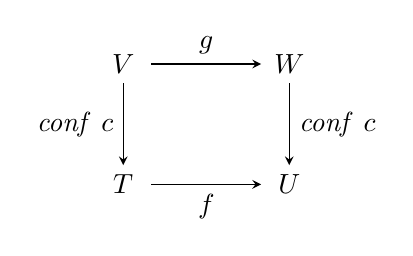
\begin{tikzpicture}
  \matrix (m) [matrix of math nodes,row sep=3em,column sep=4em,minimum width=2em]
  {
     V & W \\
     T & U \\};
  \path[-stealth]
    (m-1-1) edge node [left] {$\mathit{conf}\ c$} (m-2-1)
            edge node [above] {$g$} (m-1-2)
    (m-2-1.east|-m-2-2) edge node [below] {$f$}
             (m-2-2)
    (m-1-2) edge node [right] {$\mathit{conf}\ c$} (m-2-2)
            ;
\end{tikzpicture}
\end{center}

\section{Motivation}

In order to take advantage of the benefits of sharing provided by choices, we must develop variational
models of execution for a given language. We begin by showing that defining variational execution in a pure,
side-effect free evaluation context is a fairly straight-forward exercise before turning to the much more
difficult problem of variational execution with side effects.

\subsection{Pure variational execution}

If we do not have to worry about side effects in our language that we wish to introduce variation to
our task is comparatively easy. We begin by considering a simple arithmetic expression language
defined by the following Haskell datatype:

\begin{program}
data Arith = N Int | Add Arith Arith | Mul Arith Arith
\end{program}

In the non-variational setting we can easily define an interpreter for this language which produces
values of type \prog{Int}:

\begin{program}
eval :: Arith -> Int
eval (N i) = i
eval (Add l r) = eval l + eval r
eval (Mul l r) = eval l * eval r
\end{program}

The process of ``variationalizing" this small example is quite straightforward. First, we add a
constructor to support choices in our language:

\begin{program}
data Arith = N Int | Add Arith Arith | Mul Arith Arith | AChc Dim Arith Arith
\end{program}

Next we modify our interpreter. Instead of returning plain values of type \prog{Int},
we now return \emph{variational} values of type \prog{FTree Int}. We then take the cases
from the non-variational interpreter and make them variational by situating them within the
applicative functor instance for \prog{FTree} we defined in Section 2. Finally, we add a case
that handles our new \prog{AChc} constructor and we have completed the conversion of our
interpreter:

\begin{program}
eval :: Arith -> FTree Int
eval (N i) = pure i
eval (Add l r) = (+) <$> eval l <*> eval r
eval (Mul l r) = (*) <$> eval l <*> eval r
eval (AChc d l r) = Chc d (eval l) (eval r)
\end{program}

This basic pattern of ``variationalizing" a language by re-situating the
plain interpreter within the applicative functor for choices works well for any language that is pure
and side-effect free. The only area of concern is associated with the use of data structures in the
interpretation of the language, which often benefit from being replaced with custom variational data structures that
provide greater sharing and efficiency. Recent work has explored the benefits of custom variational
data structures for maps \cite{erictodo}, linked lists \cite{karltodo}, and stacks \cite{mengtodo}.
As such, exercising proper care in the selection and integration of variational data structures
into a variational interpreter resolves this issue.

Nevertheless, even with the support of more efficient
variational data structures, our basic pattern of converting a plain interpreter to a variational one
encounters significant difficulties in the presence of a language with side effects.

\subsection{Exceptions}

Exceptions are a common type of effect that proves challenging in a variational setting.
Consider the following program:

\begin{algorithmic}
\STATE $y \coloneqq$ getSecret()
\IF{$y$ is true}
\STATE{\textbf{throw} $e$}
\ENDIF
\STATE{$x \coloneqq$ expensiveFn()}
\end{algorithmic}

In a non-variational context, the behavior of this program should be clear.
If the variable $y$ evaluates to \textbf{true}, then an error is thrown with value
$e$. At this point evaluation should stop, meaning that the variable $x$ is never
assigned in the final statement, avoiding the costly computation of \prog{expensiveFn}. This effect of halting execution and
returning an error value is the essence of exceptions in non-variational settings.

Now we consider the behavior of the same program in a variational context.
Suppose that the variable $y$ evaluates to the variational value
$\tagtree{A}{true}{false}$. This means that in the left alternative of $A$ we
would evaluate the body of the if statement, while ignoring it otherwise. Therefore,
in the left alternative of $A$ we throw an exception, but otherwise we continue on to the
final statement.

Clearly maintaining the same behavior from the non-variational setting in the variational setting
violates correctness. If we halt execution whenever an exception is
thrown in any variant, then we also stop the evaluation of variants that never encountered an error,
as in our example for the case $\neg A$. Correctness dictates that variants that never encountered
an exception should complete their execution uninhibited.

We also can't simply continue evaluation
in every variant regardless of whether or not we have encountered an error.
Suppose that calling \texttt{expensiveFn} normally would evaluate to the variational value $\tagtree{A}{1}{2}$, but at considerable computational cost in both alternatives.
Because we know that the left alternative of $A$ will ultimately evaluate to the thrown exception $e$, we would
like to avoid the cost involved in computing the value $1$ that we will just throw away later, mirroring how throwing an exception short-circuits evaluation in the
non-variational setting. 

Another problem concerns how to keep track of which variants are in error states and what
the error values are. If we want to avoid the cost of pointless evaluation in variants that are in an error
state, we must have some efficient way of determining when evaluation is about to enter such a variant.
In the non-variational context we have no need to store and remember error values during evaluation
because we simply return the error value immediately when it is thrown. In the variational context, we
must now store these values while we continue to evaluate variants that are not in an error state.

\bibliographystyle{plain}
\bibliography{paper}















\end{document}